\newpage
\section{Continuous RL Controller Design}
\label{sec:rl_controller_design}

\subsection{Reinforcement Learning Framework}
In Reinforcement Learning, the flight controller acts as an \emph{agent} interacting with the simulated flight environment through a continuous feedback loop \cite{vankampen2025lecture, sutton2018reinforcement}. At each time step $t$, the agent receives a state observation $s_t$ from the environment, selects a continuous control action $u_t$, and receives a scalar reward $r_t$ alongside the next state $s_{t+1}$.

The goal of the agent is to learn an optimal policy $\pi(u \mid s)$ that maximizes the expected cumulative discounted future reward, known as the \emph{value function} $V(s)$ \cite{vankampen2025lecture}:
\begin{equation}
    V(s) = \mathbb{E} \left[ \sum_{k=0}^{\infty} \gamma^k r_{t+k+1} \; |\; s_t = s \right],
    \label{eq:value_function}
\end{equation}
where $\gamma \in [0, 1)$ is the discount factor specifying how much future rewards are valued relative to immediate rewards. Using the recursive Bellman property, the value function satisfies \cite{vankampen2025lecture}:
\begin{equation}
    V(s) = \mathbb{E} \left[ r_{t+1} + \gamma V(s_{t+1}) \; | \; s_t = s \right].
    \label{eq:bellman_equation}
\end{equation}

\subsection{Actor-Critic Architecture and Function Approximation}
For simple discrete tasks, value functions can be stored in lookup tables (e.g., standard Q-tables). However, discretizing a continuous 9-dimensional state space and a 2-dimensional continuous action space creates an intractable curse of dimensionality. For continuous flight control, function approximators such as Artificial Neural Networks (ANNs) are necessary \cite{vankampen2025lecture}.

In this context, an \textbf{Actor-Critic} (or Adaptive Critic Design) architecture with to distinct ANNs is utilized:
\begin{itemize}[leftmargin=*,label=$\bullet$]
    \item \textbf{Critic Network ($V_\phi$):} Approximates the value function $V(s)$. The network takes the 9-dimensional state vector as input and outputs a single scalar estimating the expected future return of that state.
    \item \textbf{Actor Network ($\pi_\theta$):} Represents the control policy mapping states directly to continuous actions. The network takes the 9-dimensional state vector and parameterizes a Gaussian distribution $\mathcal{N}(\mu(s), \sigma^2)$, outputting the mean action $\mu(s)$ and a trainable standard deviation $\sigma$ for each control channel.
\end{itemize}
Both the Actor and Critic networks are implemented as Multi-Layer Perceptrons (MLPs) with two fully connected hidden layers of 128 neurons each\footnote{This architecture aligns with standard, benchmarked configurations in prominent reinforcement learning frameworks such as those in Stable-Baselines3 \cite{raffin2021stable}. A $128\times 128$ hidden layer size is widely utilized to balance function approximation capacity with training stability and sample efficiency.} and Hyperbolic Tangent ($\tanh$) activation functions.

% \begin{figure}[H]
%     \centering
%     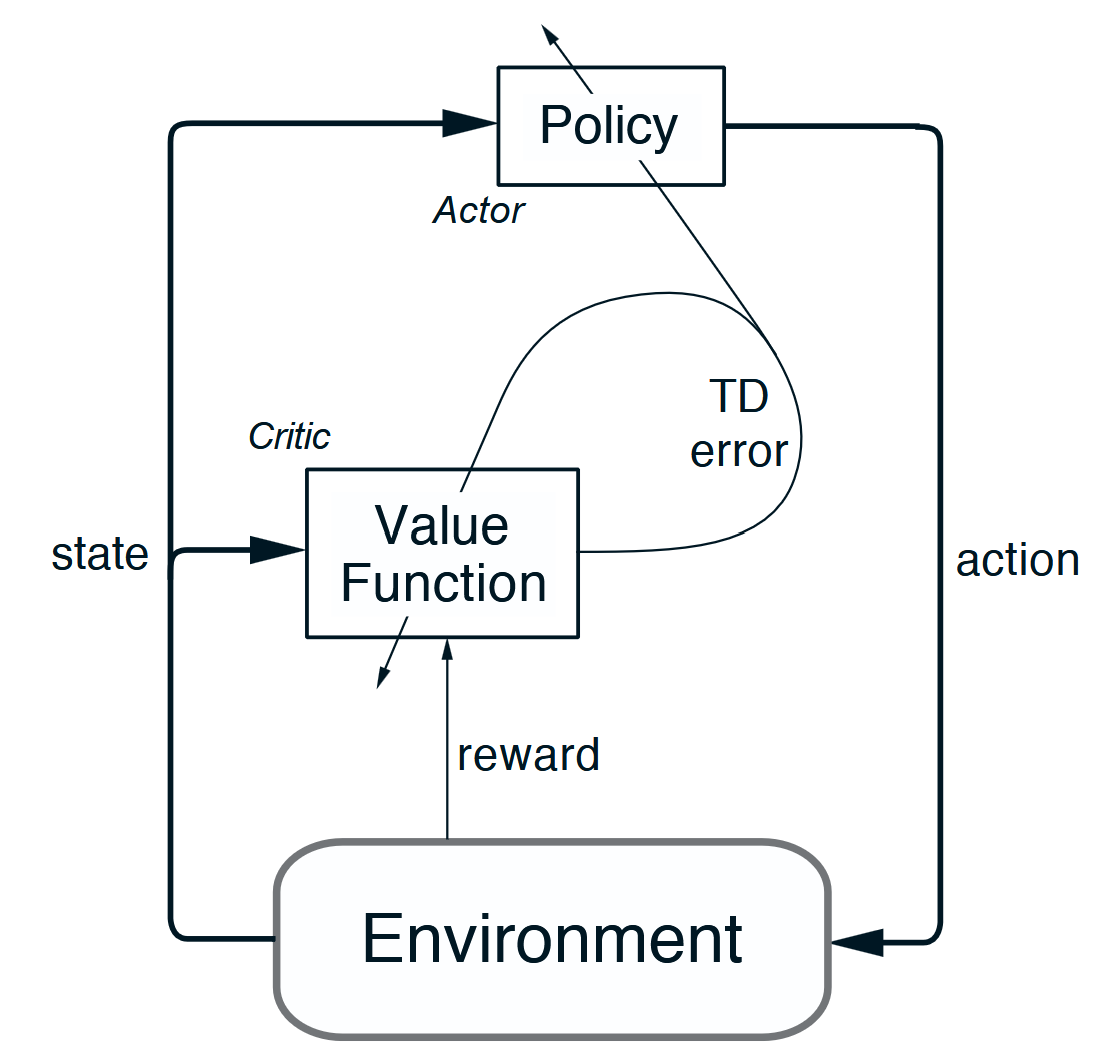
\includegraphics[width=0.45\linewidth]{figures/AC_architecture.png}
%     \caption{The actor-critic architecture \cite{sutton2018reinforcement}.}
%     \label{fig:AC_architecture}
% \end{figure}

\subsection{Proximal Policy Optimization (PPO)}
Standard actor-critic algorithms can suffer from high training instability if a gradient step causes a large, destructive policy update. Proximal Policy Optimization (PPO) \cite{schulman2017proximal} resolves this by clipping the policy probability ratio $r_t(\theta) = \frac{\pi_\theta(u_t \mid s_t)}{\pi_{\theta_{\text{old}}}(u_t \mid s_t)}$:
\begin{equation}
    L^{\text{CLIP}}(\theta) = \hat{\mathbb{E}}_t \left[ \min\left( r_t(\theta)\hat{A}_t, \, \text{clip}(r_t(\theta), 1-\epsilon_{\text{clip}}, 1+\epsilon_{\text{clip}})\hat{A}_t \right) \right],
    \label{eq:ppo_clip}
\end{equation}
with clipping parameter $\epsilon_{\text{clip}} = 0.20$. The advantage function $\hat{A}_t$ is calculated using Generalized Advantage Estimation (GAE) \cite{schulman2015high} with $\lambda = 0.95$, which measures how much better taking action $u_t$ in state $s_t$ was compared to the average expected return.

The complete PPO loss is then a combination of the clipped policy objective, the Critic value function error, and an entropy exploration bonus:
\begin{equation}
    L^{\text{PPO}}(\theta, \phi) = -\hat{\mathbb{E}}_t \left[ L^{\text{CLIP}}(\theta) - c_v (V_\phi(s_t) - R_t)^2 + c_{\text{ent}} \mathcal{H}(\pi_\theta(\cdot \mid s_t)) \right],
    \label{eq:ppo_total_loss}
\end{equation}
where $c_v = 0.50$ is the value loss weighting, $R_t$ is the target return and $c_{\text{ent}} \mathcal{H}(\pi_\theta(\cdot \mid s_t))$ is the entropy term (see following section).

\subsection{Continuous Exploration}
\label{sec:continuous_exploration}
In discrete RL algorithms (such as Q-learning), exploration is commonly handled using an $\epsilon$-greedy strategy, where the agent selects a random discrete action with probability $\epsilon$ and the greedy action with probability $1-\epsilon$ \cite{vankampen2025lecture}.

However, $\epsilon$-greedy cannot be directly applied to continuous flight control because of two main reasons:
\begin{enumerate}[leftmargin=*,label=\textbf{\arabic*.}]
    \item \textbf{Destabilizing Control Chattering:} Sampling completely random continuous actions across $[-1, 1]$ introduces abrupt, high-frequency control spikes. In a real-life dynamic aerospace system, such chattering causes severe attitude oscillations and doesn't actually help the agent explore meaningful trajectories because the system's momentum smooths out the small, random spikes.
    \item \textbf{Loss of Policy Gradients:} Hard random switching prevents smooth gradient backpropagation through the policy parameters  \cite{sutton2018reinforcement}.
\end{enumerate}

Instead, continuous actor-critic algorithms like PPO explore smoothly by sampling actions from the parameterized Gaussian distribution $\pi(u \mid s) \sim \mathcal{N}(\mu(s), \sigma^2)$. The exploration-exploitation trade-off is governed by the \emph{entropy} (spread) of this distribution. To prevent the policy from prematurely collapsing its exploration variance ($\sigma \to 0$) into a suboptimal local strategy, an \textbf{entropy bonus} term $c_{\text{ent}} \mathcal{H}(\pi)$ is added to the training loss function as shown in \cref{eq:ppo_total_loss}.

Ultimately, the entropy coefficient $c_{\text{ent}}$ acts as a hyperparameter that controls how much the agent is encouraged to explore different throttle combinations during early training while smoothly transitioning to deterministic, fine-tuned control as learning progresses. In literature, this coefficient typically spans a range between \(0\) and \(0.05\), with the original PPO benchmarks utilizing a baseline value of \(0.01\) to actively avoid premature policy convergence \cite{schulman2017proximal}.
